\documentclass[a4paper]{jpconf}
\usepackage{graphicx}
\graphicspath{{Pic/}}
\usepackage{amsmath}
\newcommand{\specialcell}[2][c]{%
  \begin{tabular}[#1]{@{}c@{}}#2\end{tabular}}
\begin{document}
\title{$3D$ model of deflection of an asymmetrical needle during motion in soft tissues}

\author{V.G. Druzhinin $^1$, V.A. Morozov$^1$}

\address{$^1$Department of Physical Mechanics, St. Petersburg University, 7/9 Universitetskaya Emb.,St Petersburg 199034, Russia}


\ead{vasily.dr.mob@gmail.com, v.morozov@spbu.ru}

\begin{abstract}
This study describes a mathematical model of deflection of a steel medical injection needle during its motion in the soft tissue phantom (imitation of human tissues). This model is necessary for adjustment of robotically assisted systems during brachytherapy procedures or similar operations where high precision needle tip positioning is prerequisite. Since the needle tip is asymmetrical, the needle will deform when moving in human tissues and consequently deflect from the rectirectilinear motion. Thus, by inserting and rotating the needle around its axis the needle tip can be led along the predetermined path. This study adopts a new approach to describe an external impact on the needle when it moves inside human tissues and also describes $2D$ and $3D$ models, a process of selection of coefficients for 3D models, and provides simulation results.
\end{abstract}

\section{Introduction}
Nowadays, robots have been increasingly replacing human manual labour. Not only can machines perform monotonous shop-floor actions but also relieve a human of more complex operations. Minimal invasive and full scale medical operations may serve as an example. This study addresses brachytherapy procedures for prostate cancer. As of today, we have developed a robotically assisted system ``OncoROBOT" in the Central Research Institute of Robotic And Technical Cybernetics to conduct such operations ~\cite{one, two}. This procedure is conducted by insertion of radiation micro-sources into the prostate gland as close as possible to the tumor.  The major challenge is to lead the needle tip to the target point (a tumor) during an operation. The advantages of employing robots as compared to traditional methods are that a robotically assisted manipulator can deliver higher accuracy when aiming a tool than a human, as well as control the acting force which allows not only for enhancement of the quality of the currently utilised operations but also for laying the groundwork for radically new surgical technology. Another crucial advantage is that there is no direct contact between a doctor and a radiation source which will advance safety of medical personnel against associated radiation exposure. During an operation a needle gets deformed due to its geometrical features which results in deflection from the rectilinear motion. The study ~\cite{Model} illustrates development stages  of model, highlights existing methods and approaches, and shows a $2D$ model describing deflection of a needle when it is moving inside human soft tissues. This research will solve the task of needle positioning within coordinates $Oxyz$ and address enhancement of model accuracy. The needle moves by rotating around its axis. In this case, the needle tip rotates together with the plane of arc curvature thereby controlling the direction of its further motion. When the needle is being inserted along the rectilinear path it shall be constantly rotating. The developed model may be used for developing ``MPC-controllers" i.e. systems based on model predictive control. For instance, the study ~\cite{four} shows a development process of such a system, however, the authors used another approach to simulation. They ~\cite{four} used the Lagrange equation to position the needle tip. Besides, experiment conditions and the needle itself were quite different from those described herein.

The study ~\cite{five} illustrated  propose a finite-dimensional mathematical model of a mechatronic system using a piezoelectric drive to move a needle along a given straight line. The study ~\cite{six} , a similar approach is used, the force of external influence is modeled in a different way.

The study ~\cite{seven} illustrated the series of experiments are performed to explore the effect of influence factors  on the insertion force. Different tissues such as skin, muscle, fat, liver capsule and vessel are proved to generate various force cures, which can contribute to the judgement of the needle position and provide efficient insertion strategy.

\section{Model}
\subsection{2D model}

Thus, it is necessary to investigate a model which predicts and adjusts the needle motion inside human tissues. We have selected a steel medical injection needle with a length of 100 mm and a diameter of 1 mm with various tip angles (Figure  \ref{n1}) as a model object. We shall look into the force balance equation to develop a model of the needle motion ~\cite{Model}:

\begin{equation} \label{eq1}
\vec{F}_{needle} = \vec{F_{t}} + \vec{F_{f}} + \vec{w}(x),
\end{equation}
where $\vec{F_{t}}$ is the force acting on the needle tip, $\vec{F_{f}}$ is the friction, $\vec{w}(x)$ is distributed load and $\vec{F}_{needle}$ is the force with which the needle is inserted.

\begin{figure}[h]
\center{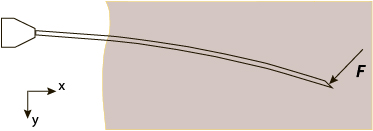
\includegraphics[scale=0.8]{n1.jpg}}
\caption{Needle shape, $F$ is the medium reaction}
\label{n1}
\end{figure}

This research addresses the problem as follows:

\begin{equation} \label{eq2}
\vec{F}_{needle} = \vec{F_{t}}.
\end{equation}

To solve the problem and calculate the deflection of the needle tip and the deflection angle we will use the equations ~\cite{Model}:
\begin{equation} \label{eq3}
y_{n} = Fl(t)^3 / 3EJ_{x},
\end{equation}

\begin{equation} \label{eq4}
\theta = Fl(t)^2 / 2EJ_{x},
\end{equation}
where  $n$ is the current iteration of simulation, $y_{n}$ is the deflection of the needle tip at the current time step,
$F$  is the force acting on the needle tip (Fig.  \ref{n1}), $J_{x}$  is the axial moment of inertia, 
$l(t)$  is the length of the needle in human tissues, $t$  is the time, $E$  is the Young's modulus, $\theta$  is the deflection angle.

To simulate external force $F$ acting on the needle when it moves inside the human tissues we will use the head drag force:

\begin{equation} \label{eq5}
F = C (\rho v^2/2) S, 
\end{equation}
where  $C$  is the drag coefficient, $\rho$  is the density of tissue, $v$  is the velocity of the needle motion, $S$  is the reference area of the body, $S = V^{(2/3)}$, where $V = (\pi d^2/4)l$ is the needle volume  in human tissues, $d$ is needle diameter, $l$ is the length of the needle in human tissues.

To calculate the needle deflection using equations \eqref{eq3} and \eqref{eq4} we should consider the projection of force F on the perpendicular to the needle axis. In this formulation of the problem according to proposed equations \eqref{eq3}, \eqref{eq4} and \eqref{eq5}, we will calculate the deflection iteratively summing up its previous steps. Thus we shall retain the deflection at each step of simulation:

\begin{equation} \label{eq6}
y_{all} = \sum\limits_{1}^{n-1} y_{n},
\end{equation}
where $n$  is the current iteration of simulation, $y_{all}$  is the total deflection of the needle during its motion in human tissues, $y_{n}$  is the deflection of the needle tip at the current time step.

\subsection{3D model}

For the $3D$ model we will use a system of coordinates given in Figure  \ref{n2}. In this case, the rotation angle is the value by which the needle shear plane rotates.

\begin{figure}[h]
\center{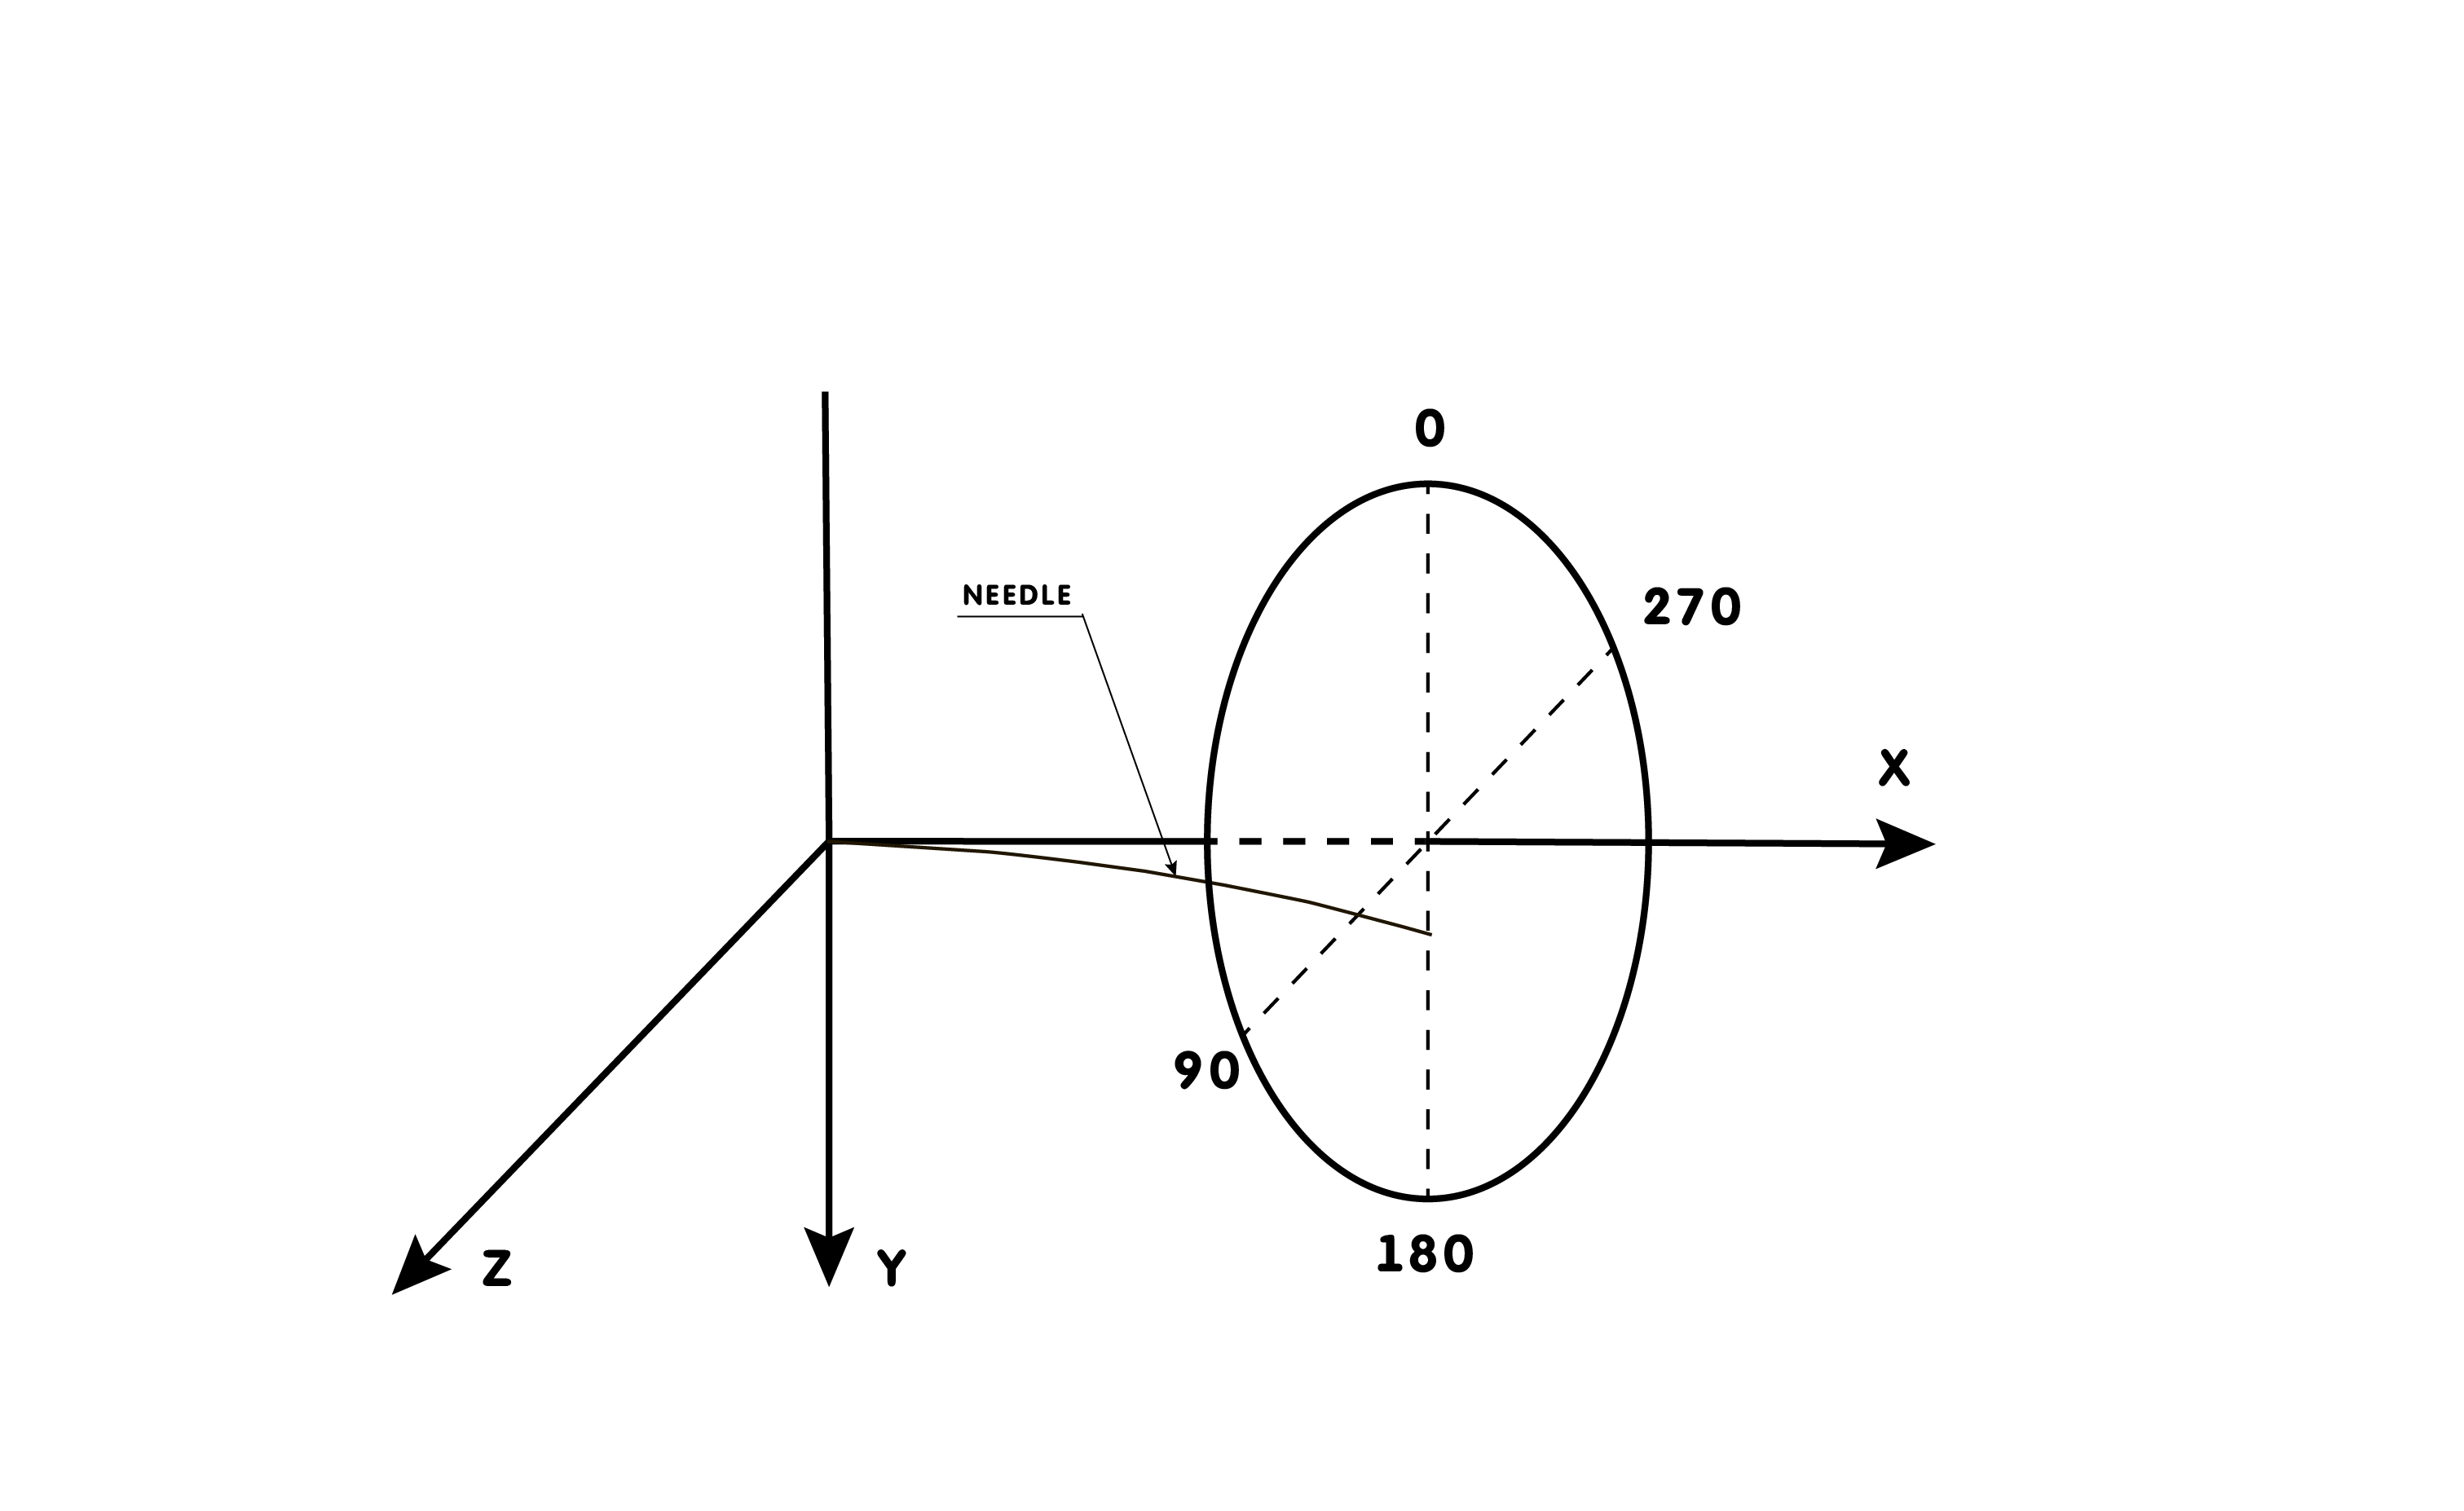
\includegraphics[scale=0.5]{n2.jpg}}
\caption{System of coordinates under consideration}
\label{n2}
\end{figure}

To calculate the position of the needle tip we will use the following equations:

\begin{equation} \label{eq7}
z_{n} = 
 \begin{cases}
   y_{n} sin(\gamma) &{ 0 \leq \gamma \leq \pi/2 }\\
   y_{n} sin(\pi - \gamma) &{ \pi/2 \leq \gamma \leq \pi }\\
  - y_{n} sin( \gamma - \pi) &{ \pi \leq \gamma \leq 3\pi/2 }\\
   - y_{n} sin(2\pi -  \gamma) &{ 3\pi/2 \leq \gamma \leq 2\pi }\\
 \end{cases}
\end{equation}

\begin{equation} \label{eq8}
z_{all} = \sum\limits_{1}^{n} z_{n},
\end{equation}

\begin{equation} \label{eq9}
y_{k} = 
 \begin{cases}
   y_{n} cos(\gamma) &{ 0 \leq \gamma \leq \pi/2 }\\
   - y_{n} cos(\pi - \gamma) &{ \pi/2 \leq \gamma \leq \pi }\\
  - y_{n} cos( \gamma - \pi) &{ \pi \leq \gamma \leq 3\pi/2 }\\
    y_{n} cos(2\pi -  \gamma) &{ 3\pi/2 \leq \gamma \leq 2\pi }\\
 \end{cases}
\end{equation}

\begin{equation} \label{eq10}
y_{all} = \sum\limits_{1}^{k} y_{k},
\end{equation}
where  $\gamma$  is the angle by which the needle rotated around its axis in 1 simulation step., $z_{all} $  is the deflection component along axis $Oz$, $y_{all}$  is the deflection component along axis $Oy$, $y_{n}$  is the deflection per 1 simulation time step.

To calculate the total deflection from axis $Ox$ we will use the following equation:

\begin{equation} \label{eq11}
d_{all} = \sqrt{y_{all}^2  +  z_{all} ^2}.
\end{equation}

Thus, at each step of simulation, the angle by which the needle has rotated will be analysed. Then the deflection will be calculated at each given step and converted into coordinates and from the given coordinates $y$ and $z$ the total deflection from axis $Ox$ will be calculated. Further, we will investigate the simulation results and compare it with the experimental evidence.

\subsection{Calculation of drag coefficients}
The problem to be solved is a multi-parameter one and depends on several variables, namely, translational and rotational velocities of a needle inside tissues. It is necessary to find a solution which provides minimal difference between the experimental and predicted data. $2D$ model simulation results with constant coefficient $C$ adopted from the book of reference outlined rather significant errors.

Therefore, this coefficient will be introduced as some functional dependence on needle velocity of travel developed on experimental data. This approach ensured minimal errors during simulation. 

Here, we will investigate coefficients for various rotational velocities 0, 3, 4, 5 rad/s.
For the rotational velocity equal to 0 rad/s:
\begin{multline} \label{eq12}
C= 2.2293\cdot10^{11} v^6 - 2.5517\cdot10^{10} v^5+1.788\cdot10^9 v^4 - \\ -2.8053\cdot10^7 v^3 +3.6420\cdot10^5 v^2-2.4583\cdot10^3 v+7.4299.
\end{multline}

For the rotational velocity equal to 3 rad/s:
\begin{multline} \label{eq13}
C= -6.1243\cdot10^{18} v^9 + 1.0095\cdot10^{18}v^8 -  7.2393\cdot10^{16} v^7 +\\+ 2.9601\cdot10^{15} v^6 - 7.5961\cdot10^{13} v^5 + 1.2673\cdot10^{12} v^4 - \\-1.3740\cdot10^{10} v^3 + 9.3490\cdot10^7 v^2 - 3.6459\cdot10^5 v+ 634.2858.
\end{multline}

For the rotational velocity equal to 4 rad/s:
\begin{multline} \label{eq14}
C= -5.5744\cdot10^{18} v^9 + 9.29\cdot10^{17}v^8 -  6.7439\cdot10^{16} v^7 +\\+ 2.7959\cdot10^{13} v^6 - 7.2889\cdot10^{13} v^5 + 1.2385\cdot10^{12} v^4 - \\-1.3720\cdot10^{10} v^3 + 9.5768\cdot10^7 v^2 - 3.3892\cdot10^5 v+ 693.0468.
\end{multline}

For the rotational velocity equal to 5 rad/s:
\begin{multline} \label{eq15}
C= -1.5127\cdot10^{19} v^9 + 2.4827\cdot10^{18}v^8 -  1.7730\cdot10^{17} v^7 +\\+ 7.2242\cdot10^{15} v^6 - 1.8491\cdot10^{14} v^5 + 3.082\cdot10^{12} v^4 - \\-3.3464\cdot10^{10} v^3 + 2.2881\cdot10^7 v^2 - 9.0014\cdot10^5 v+ 1.5829\cdot10^3.
\end{multline}

Table \ref{table1}  shows the results of calculated coefficients for various translational and rotational velocities according to equations \eqref{eq12}, \eqref{eq13}, \eqref{eq14}, \eqref{eq15}.

\begin{table}[h]
\caption{Head drag coefficient}
\label{table1}
\begin{center}
\begin{tabular}{ | c | c | c | c | c | }
\hline
 & \multicolumn{4}{c|}{Coefficients $C$}   \\ 
 \cline{2-5}
 \raisebox{1.5ex}[0cm][0cm] {\specialcell{Linear \\ velocity, mm/s }} & 0 rad/s & 2 rad/s & 4 rad/s & rad/s \\ \hline
3   &  2.664938602	& 97.13340693	& 114.2592189	& 247.5463059 \\ \hline
6	& 1.07169768	& 15.73135406	& 19.05791457	& 38.10638623 \\ \hline
9	& 0.700671524	& 6.365846027	& 7.064884636	& 13.06272217 \\ \hline
12	& 0.659327251	& 3.23079564	& 3.700963655	& 6.112620422 \\ \hline
15	& 0.660593963	& 1.842929895	& 2.20407716	& 3.438567258 \\ \hline
18	& 0.688335976	& 1.204554851	& 1.455901558	& 2.214430941 \\ \hline
21	& 0.779838013	& 0.795031504	& 0.941747061	& 1.480803942 \\ \hline
24	& 0.925302352	& 0.559047066	& 0.662773618	& 1.06863687  \\ \hline
27	& 1.084357932	& 0.403247032	& 0.498425997	& 0.792121034 \\ \hline
30	& 1.319581413	& 0.312718332	& 0.380221049	& 0.626483873 \\ \hline
\end{tabular}
\end{center}
\end{table}

\section{Simulation results}

The simulation was run for different initial values. The following translational velocities were used during simulation: 3, 6, 9, 12, 15, 18, 21, 24, 27, 30 mm/s. The following rotational velocities were considered:
0, 3, 4, 5 rad/s. For various rotational velocities, the relevant polynomials were used to calculate the head drag coefficient. Table \ref{table2}  shows the simulation results.

\begin{table}[h]
\caption{Needle deflection from linear motion}
\label{table2}
\begin{center}
\begin{tabular}{ | c | c | c | c | c | }
\hline
 & \multicolumn{4}{c|}{deflection, mm:}   \\ 
 \cline{2-5}
 \raisebox{1.5ex}[0cm][0cm] {\specialcell{Linear \\ velocity, mm/s }} & 0 rad/s & 2 rad/s & 4 rad/s & 5 rad/s \\ \hline
3	& 0.10	& 0.17	& 0.15	& 0.26 \\ \hline
6	& 0.16	& 0.22	& 0.20	& 0.32 \\ \hline
9	& 0.24	& 0.30	& 0.25	& 0.37 \\ \hline
12	& 0.40	& 0.36	& 0.31	& 0.41 \\ \hline
15	& 0.62	& 0.40	& 0.36	& 0.45 \\ \hline
18	& 0.93	& 0.45	& 0.41	& 0.50 \\ \hline
21	& 1.43	& 0.47	& 0.42	& 0.53 \\ \hline
24	& 2.22	& 0.49	& 0.44	& 0.57 \\ \hline
27	& 3.29	& 0.50	& 0.47	& 0.60 \\ \hline
30	& 4.94	& 0.53	& 0.49	& 0.65 \\ \hline
\end{tabular}
\end{center}
\end{table}

When we using the coefficients $C$ in the form of polynomials, the difference between the results of modeling the deflection of the needle from the $Ox$ axis and the experimental data does not exceed 0.01 mm

\section{Conclusion}
In the course of this research, we have developed $2D$ and $3D$ models which describe the deflection of the medical injection needle from the linear motion when moving inside human tissues. To achieve the maximum possible approximation between the predicted and experimental data, we have calculated and selected the head drag coefficients for simulation. The model was simulated at different initial conditions. The simulation results using the calculated coefficients reflect that the given model can be used in robotic systems to predict the movement or to design ``MPC-controllers". This model can also be used for virtual operations involving injections.


\section{References}
\bigskip
\begin{thebibliography}{99}
\small
\bibitem{one}{Gryaznov N.A., Kireeva G.S., Kharlamov V.V., Nikitin  S.A. 2016 {\it Control of robot for brachytherapy based on ultrasonic sensor data} (St. Petersburg Robotics and Technical Cybernetics) pp. 67-71.}
\bibitem{two}{Gryaznov N.A., Kireeva G.S., Kharlamov V.V., Nikitin  S.A. 2017 {\it Prospects of application of original multirobotic system for brachytherapy of prostate cancer} Vol. 176, pp. 107-111.}
\bibitem{Model}{Druzhinin V.G., Morozov V.A., Nikitin S.A., Kharlamov V.V. 2018 { \it Model of the deviation of the medical needle during the movement in human tissue} (Perm, Russian Journal of Biomechanics)  pp. 459-472.}
\bibitem{four}{Fichtinger G. 2002 {\it System for robotically assisted prostate biopsy and therapy with intraoperative CT guidance} Vol. 9. pp. 60–74.}
\bibitem{five} {Goryacheva I.G., Dosaev M.Z., Selyutskiy Y.V., Yakovenko A.A., Hsiao C., Huang C., Ju M., Yeh C. 2020 { \it Control of Insertion of Indenter into Viscoelastic Tissue using a Piezoelectric Drive} pp. 304-311.}
\bibitem{six}{Khadem M., Fallahi B., Rossa  C., Sloboda  R. S.,  Usmani N. and Tavakoli M., 2015 { \it A mechanics-based model for simulation and control of flexible needle insertion in soft tissue} pp. 2264-2269.}
\bibitem{seven}{Shan Jiang, Pan Li, Yan Yu, Jun Liu, Zhiyong Yang, 2014 {\it Experimental study of
needle–tissue interaction forces: Effect of needle geometries, insertion
methods and tissue characteristics},Vol. 47, pp 3344-3353. }


\end{thebibliography}

\end{document}


